%%%%%%%%%%%%%%%%%%%%%%%%%%%%%%%%%%%%%%%%%%%%%%
%                insertmeeting
% 1) Title (something creative & funny?)
% 2) Date (MM/DD/YYYY)
% 3) Location (ex. Hagerty High School)
% 4) People/Committees Present 
% 5) Picture 
% 6) Start Time & Stop Time (ex. 12:30AM to 4:30PM)
%%%%%%%%%%%%%%%%%%%%%%%%%%%%%%%%%%%%%%%%%%%%%%
\insertmeeting 
	{Meeting Example} 
	{12/03/21} 
	{Hagerty High School}
	{Nathan, Ritam, Samantha}
	{Images/RobotPics/robot.jpg}
	{2:30 - 4:30}
	
\hhscommittee{General}
\noindent\hfil\rule{\textwidth}{.4pt}\hfil
\subsubsection*{Goals}
\begin{itemize}
    \item Prevent grabber from throwing blocks
    \item Analyze and solve other problems with intake from meet 1
   

\end{itemize} 

\noindent\hfil\rule{\textwidth}{.4pt}\hfil

\subsubsection*{Accomplishments}
Because we realized that exams were coming up and that software still needed to work on autonomous, we decided to push back the redesign of the roller intake until after the 2nd meet. Instead, we plan to use the remaining time before the meet fixing the problems with the old grabber intake and on ensuring our drivers are confident enough to maintain or increase our 2nd place position in the league.
We started out with the biggest problem we faced with the intake: throwing blocks. Whenever we would grab blocks (particularly heavy ones) then swing the arm back to get into scoring position, there was a chance that the robot would let go of the block and throw it, incurring a minor penalty. The way that we plan to deal with this is by changing out the rubber to increase the amount of friction on the block. Just switching out the rubber pad wouldn’t be sufficient on its own, so we found another way to stop the blocks from falling out. Because the rubber sheet we used before spanned the entire width of the finger, the force pushing down on the block was distributed over a larger area. Our plan is to have the rubber only on the ends of the finger distributing the force of the block over a smaller area (Figure \ref{fig:pic1}). While it may seem like friction would increase with more surface area, having a smaller surface area and thus more compression puts more force downwards on the block which is extremely helpful to keeping the block gripped in the intake (Figure \ref{fig:pic2}). Testing this out, we found it to be very effective, making it almost impossible to launch blocks.
One of the other problems we had at the first meeting about the intake was that it sometimes was able to grab 2 blocks. Because the finger is so wide, it would often come down and hold 2 blocks in place. This also contributed to the issue of throwing blocks, because the combination of poor surface area and low compression from holding 2 blocks with 1 finger made the blocks fly out of the grabber just about every time. To remedy this issue, we decreased the width of the finger by .25 inches, which in other contexts might seem small, should be enough to reduce the amount of times we grab 2 blocks enough to make the issue go away.

 

\begin{figure}[ht]
\centering
\begin{minipage}[b]{.48\textwidth}
  \centering
  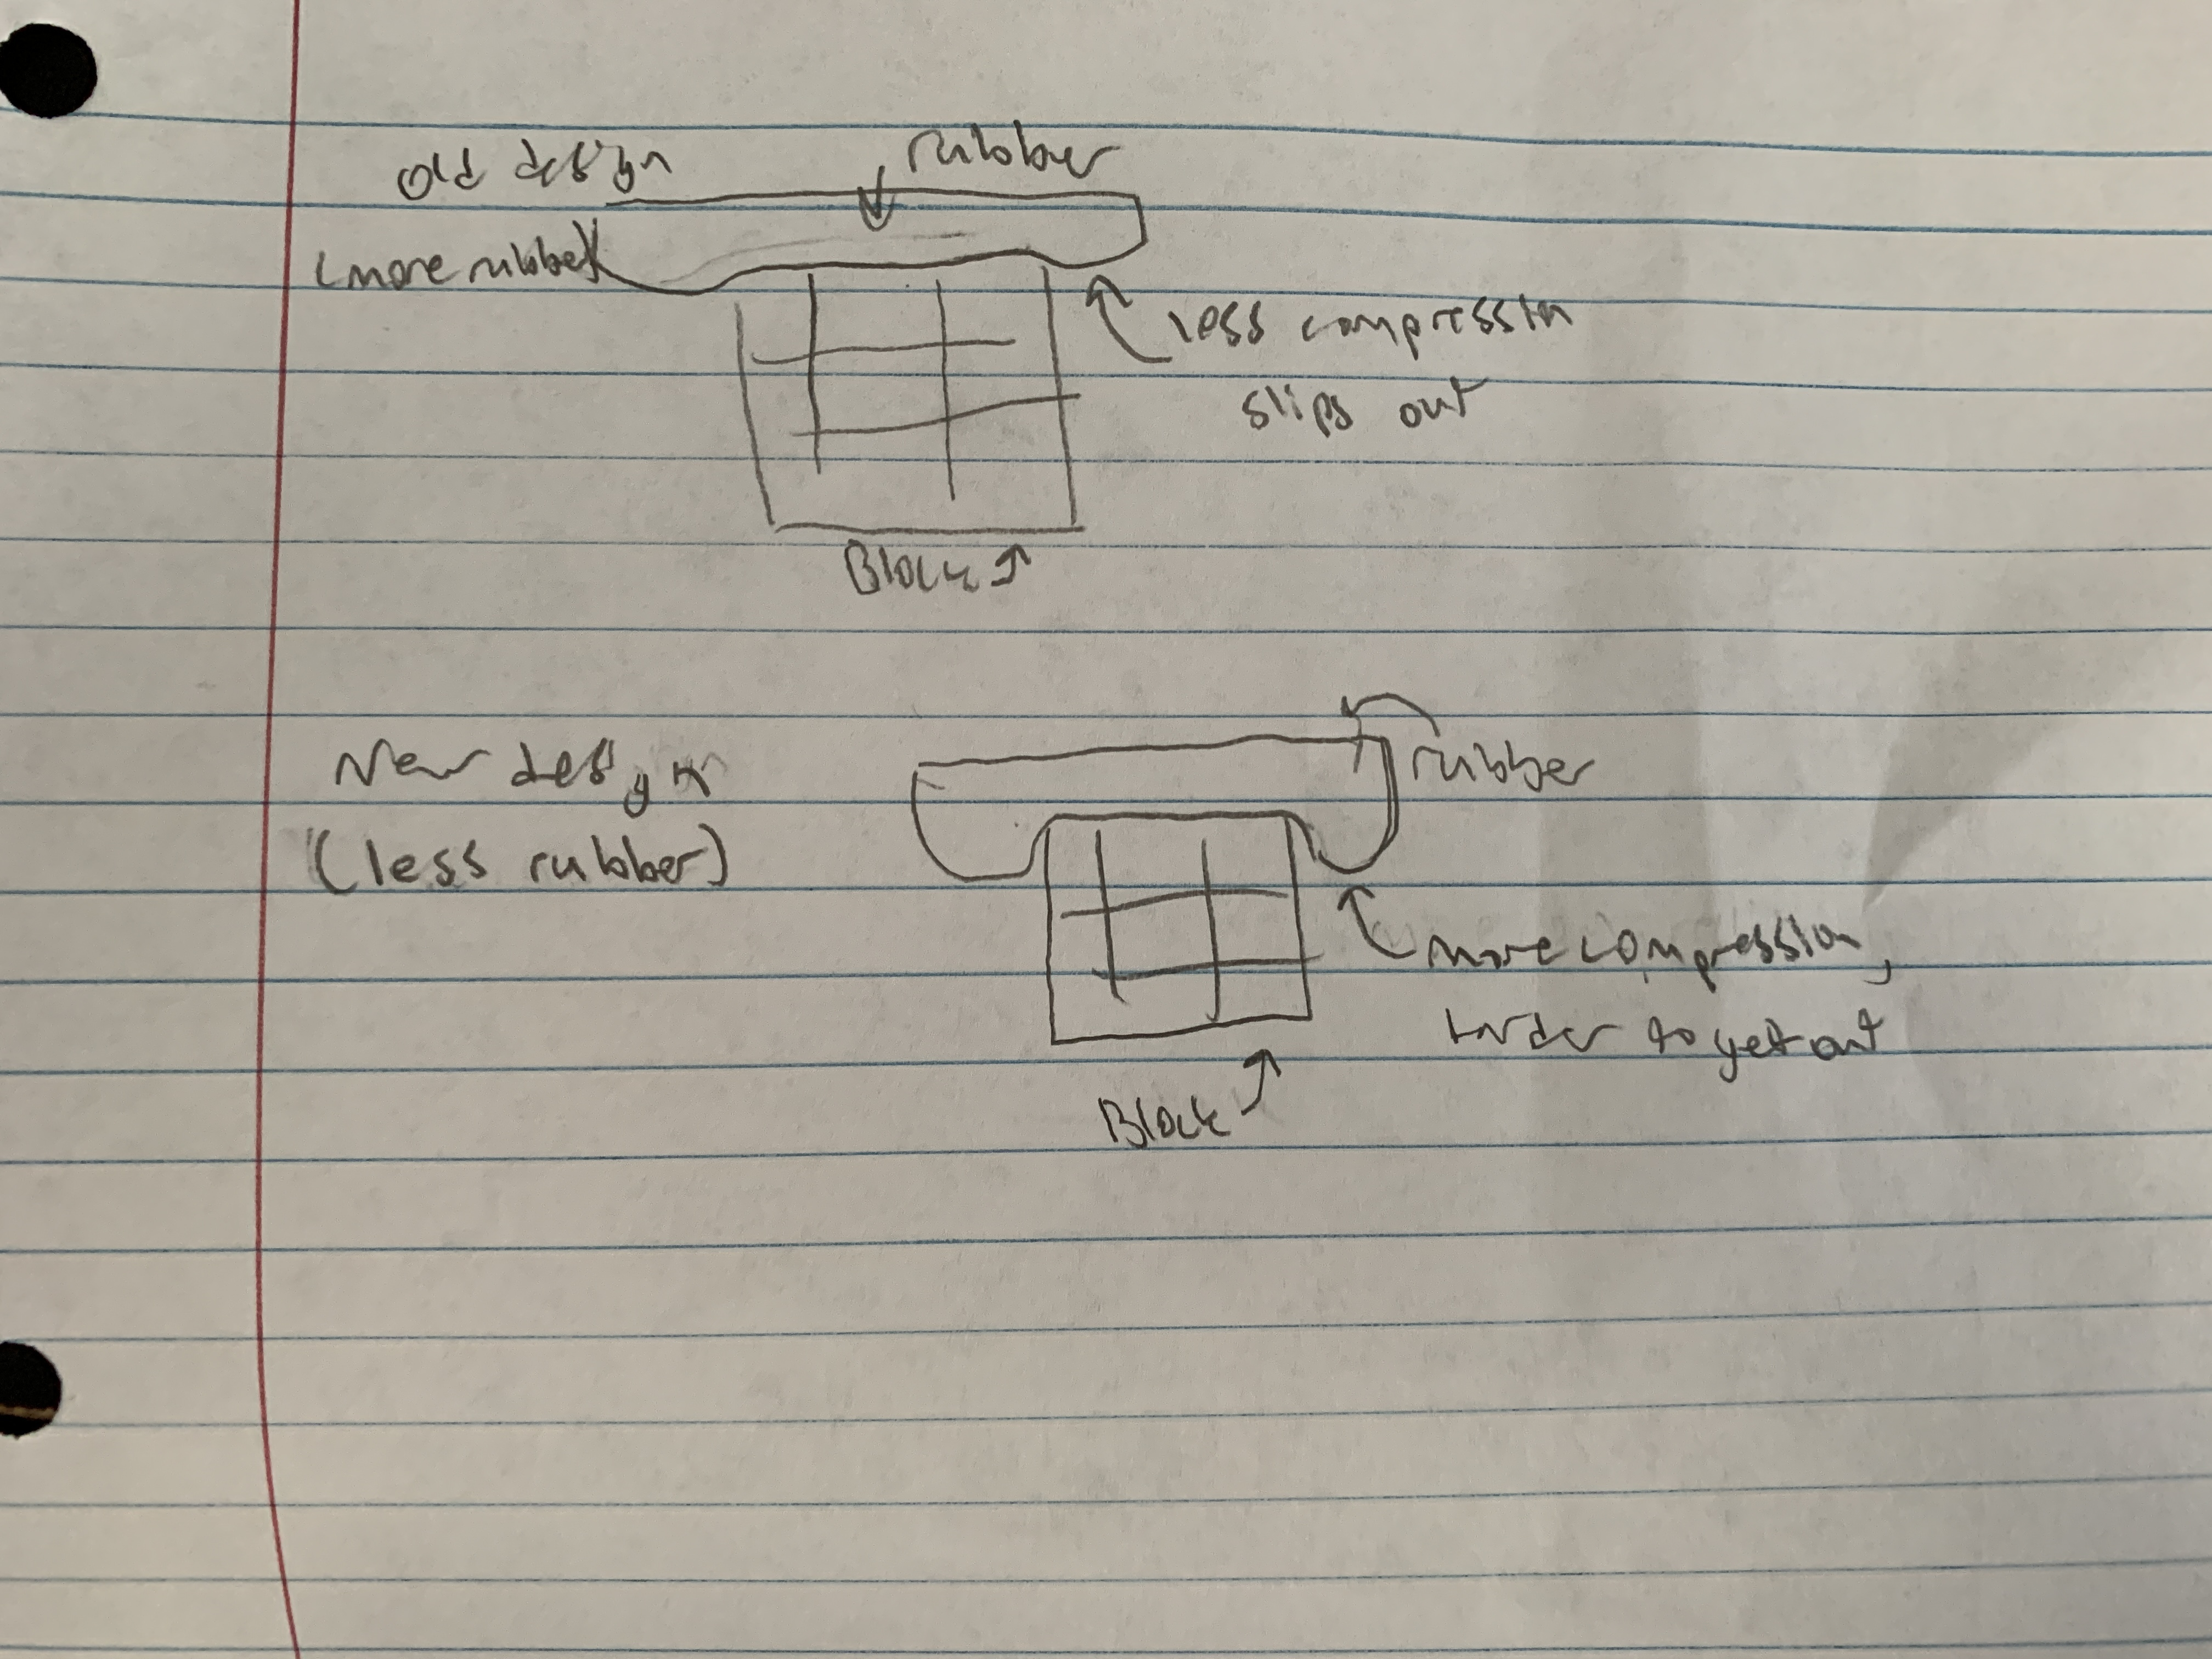
\includegraphics[width=0.95\textwidth]{Meetings/December/12-03-21/12-3-21_Hardware_Figure1 - Nathan Forrer.jpg}
  \caption{New finger sketches}
  \label{fig:pic1}
\end{minipage}%
\hfill%
\begin{minipage}[b]{.48\textwidth}
  \centering
  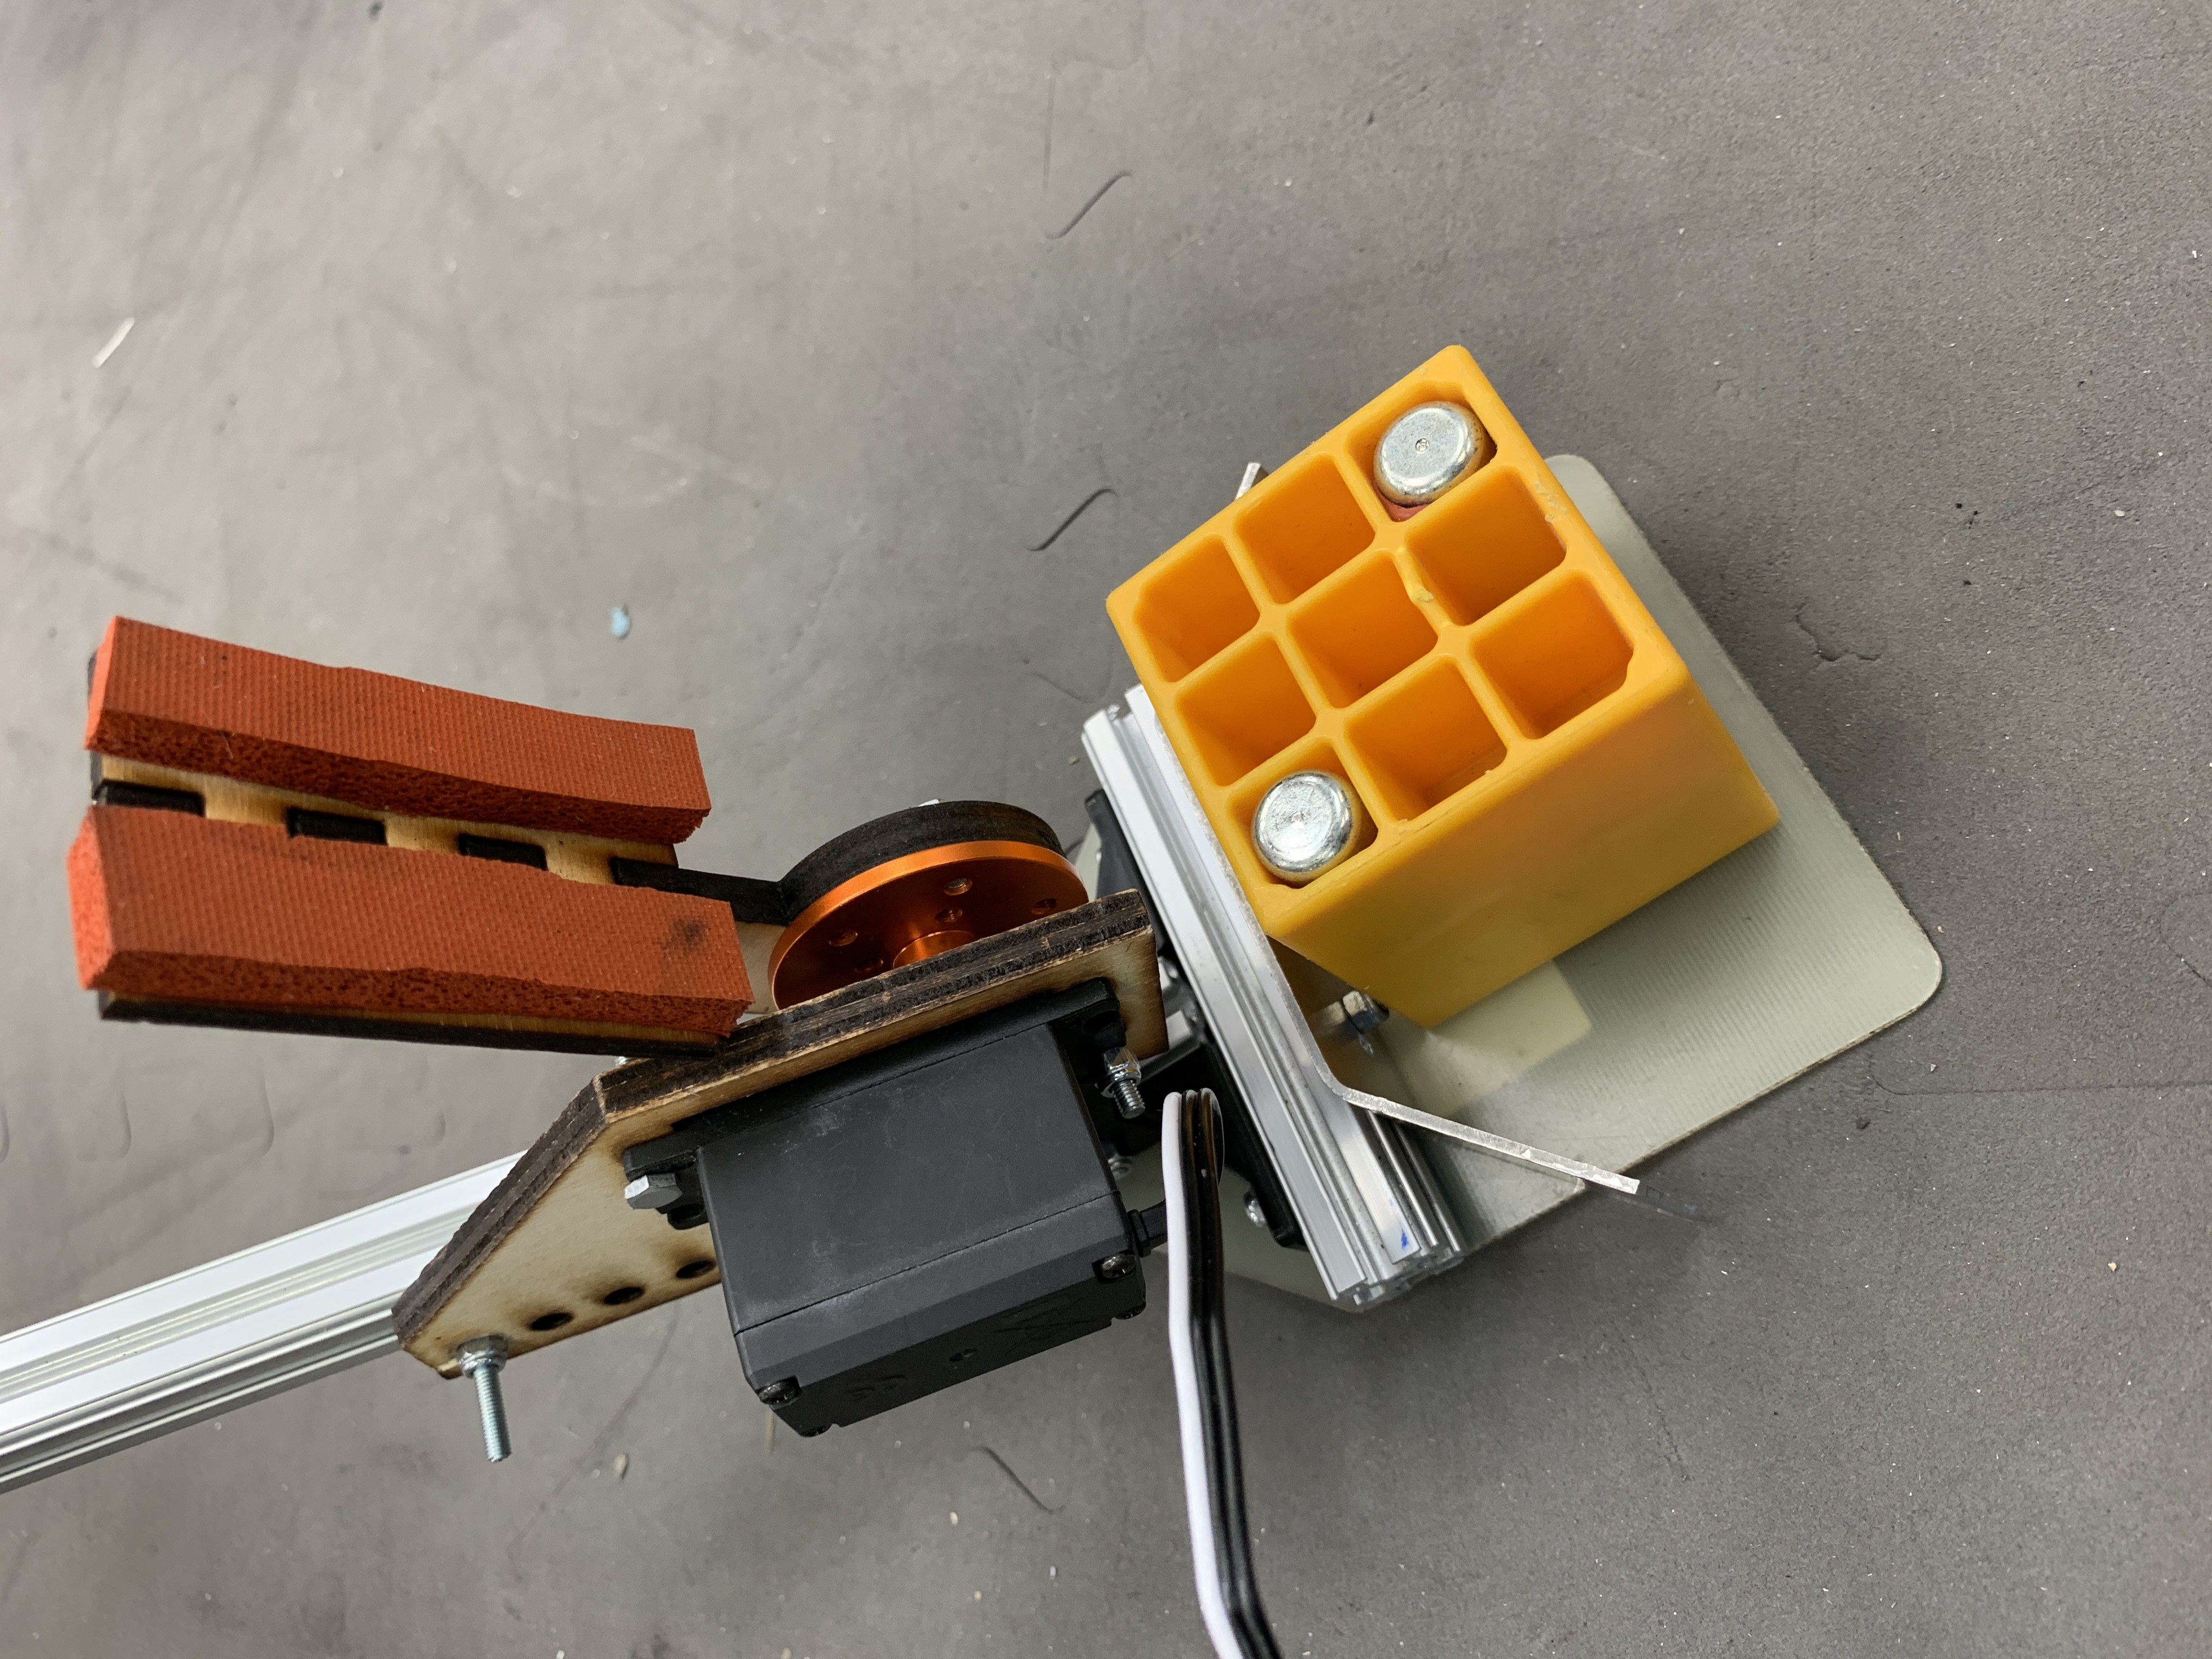
\includegraphics[width=0.95\textwidth]{Meetings/December/12-03-21/12-3-21_Hardware_figure2 - Nathan Forrer.JPG}
  \caption{The new intake in action}
  \label{fig:pic2}
\end{minipage}
\end{figure}


\whatsnext{
\begin{itemize}
    \item Do driver practice and prepare for upcoming meet
    \item Fix any hardware issues that arise before the meet

\end{itemize} 
}

